\documentclass[12pt]{article}
\usepackage[spanish,mexico]{babel}
	\selectlanguage{spanish}
\usepackage{graphicx}
\usepackage{amsmath}
\usepackage{wrapfig}
\usepackage{float}
\usepackage[utf8]{inputenc}
\usepackage{hyperref}
\usepackage{graphicx}
\graphicspath{{images/}}

\usepackage{vmargin}
\setmarginsrb{3 cm}{1.0 cm}{3 cm}{1.0 cm}{1 cm}{1.5 cm}{1 cm}{1.5 cm}
\usepackage{listings}
\usepackage[usenames,dvipsnames]{color}
	\definecolor{ocre}{RGB}{42,105,21}
	\definecolor{ocre2}{RGB}{47,109,130}
	\definecolor{gray2}{gray}{0.95}
	\lstset{
		language=Python,
		backgroundcolor=\color{gray2},
		basicstyle=\color{black}\small\ttfamily, 
		breakatwhitespace=false,         
		breaklines=true,                 
		captionpos=b,                    
		columns=flexible,
		commentstyle=\color{ocre2}\ttfamily, 
		deletekeywords={...},            
		escapeinside={\%*}{*)},          
		extendedchars=true,             
		frame=single,	                 
		keepspaces=true,                 
		keywordstyle=\color{blue}\bfseries,       
		otherkeywords={*,...},          
		numbers=left,                    
		numbersep=5pt,                   
		numberstyle=\tiny, 
		rulecolor=\color{black},         
		showspaces=false,                
		showstringspaces=false,          
		showtabs=false,                  
		stepnumber=1,                    
		stringstyle=\normalfont\color{ocre},     
		tabsize=2,	                     
		title=\lstname                  
		}

\title{Actividad 10: Animaciones con Matplotlib}
\author{Martin Alejandro Paredes Sosa}
\date{Marzo, 2016}

\begin{document}
\maketitle

\section{Introducción}
\noindent
La matemática de un péndulo simple es, en general, compleja. Hacer suposiciones que simplifican la descripción nos permite resolver analíticamente las ecuaciones de movimiento. El péndulo simple, es una idealización se un péndulo real, pero en un sistema aislado donde se asume:
\begin{itemize}
	\item La cuerda tiene una masa despreciable, es rígida y se mantiene tensa.
	\item El péndulo se maneja como una masa puntual.
	\item El movimiento es en dos dimensiones trazando un arco.
	\item No pierde energía por fricción o resistencia al aire.
	\item El campo gravitacional es uniforme.
	\item El soporte no se mueve.
\end{itemize}

La ecuación diferencial que representa el movimiento de un péndulo simple es:
\begin{equation}\label{EcDf}
	\frac{d^2\theta}{dt^2} + \frac{g}{\ell}\sin\theta = 0
\end{equation}
donde $g$ es la aceleración de la gravedad, $\ell$ es la longitud del péndulo y $\theta$ es el angulo de desplazamiento \cite{PendWiki}.

En esta práctica se nos pidió realizar una animación de un péndulo utilizando la biblioteca de \texttt{Matplotlib}.Haciendo uso del código de Jake Vanderplas para el péndulo doble \cite{cod1} y el código de Matplotlib de subplots\cite{cod2}, se crearon las animaciones del péndulo y su espacio fase.


\section{Ejercicio y Resultados}
Esta actividad consistió en realizar un código en python que nos permitiera construir una animación del péndulo simple. Se hizo uso de la librería \emph{matplotlib.animation} para crear la animación y poder observar el movimiento del péndulo con diferentes condiciones iniciales. \\

Los códigos que se utilizaron fueron los siguientes:
\lstinputlisting[caption={Código Animacion\_Fase.py}]{Animacion_Fase.py}
\lstinputlisting[caption={Código Animacion\_Pendulo.py}]{Animacion_Pendulo.py}
El resultado que se obtuvo fue el siguiente:

\begin{figure}[H]
\centering
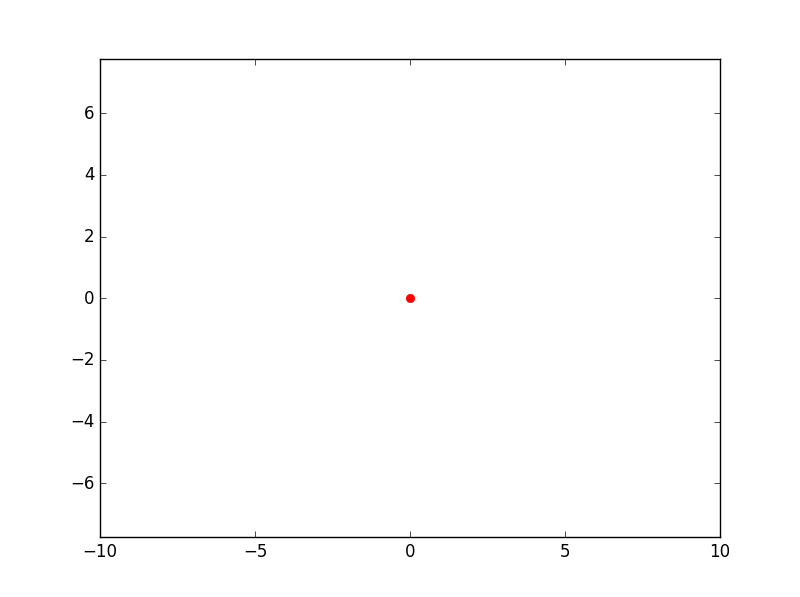
\includegraphics[width=7cm]{Fase0.png}
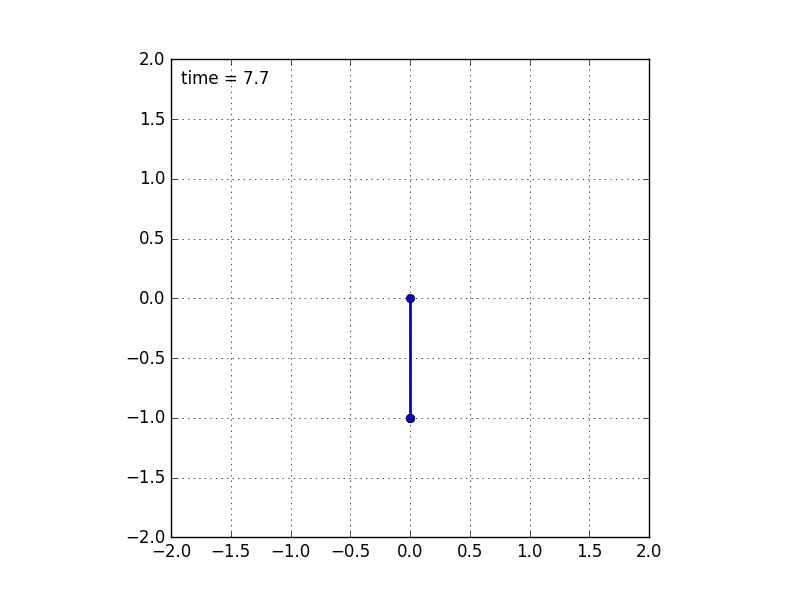
\includegraphics[width=7.5cm]{Pendulo0.png}
\caption{Imagen de Animación de péndulo con ángulo inicial 0.}
\end{figure}

\begin{figure}[H]
\centering
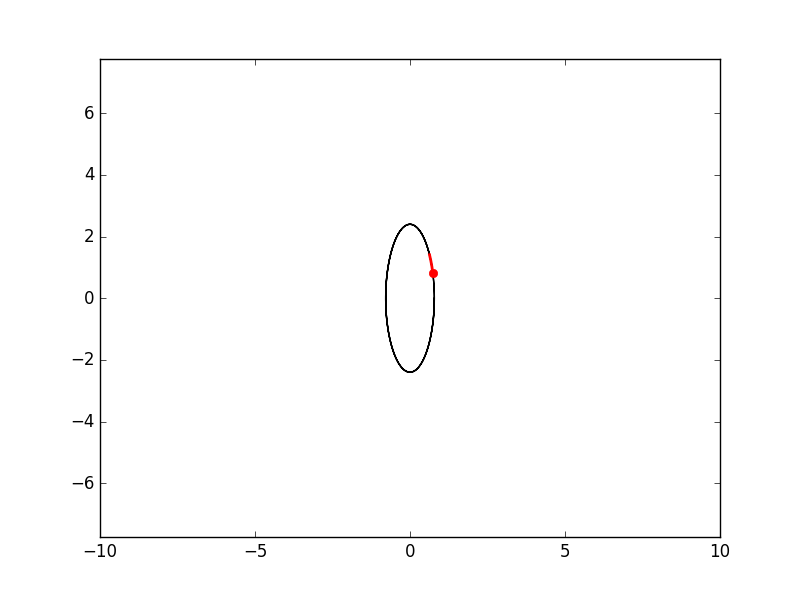
\includegraphics[width=7cm]{Fase45.png}
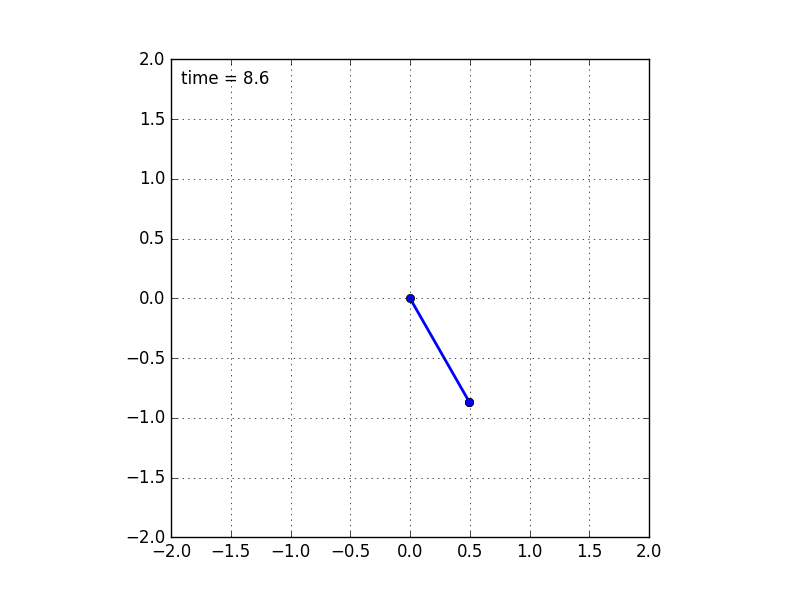
\includegraphics[width=7.5cm]{Pendulo45.png}
\caption{Imagen de Animación de péndulo con ángulo inicial 45.}
\end{figure}

\begin{figure}[H]
\centering
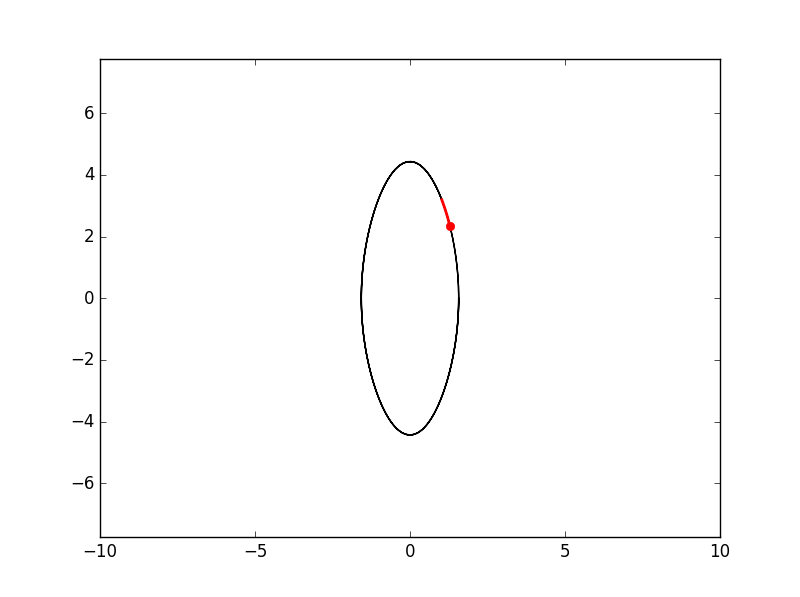
\includegraphics[width=7cm]{Fase90.png}
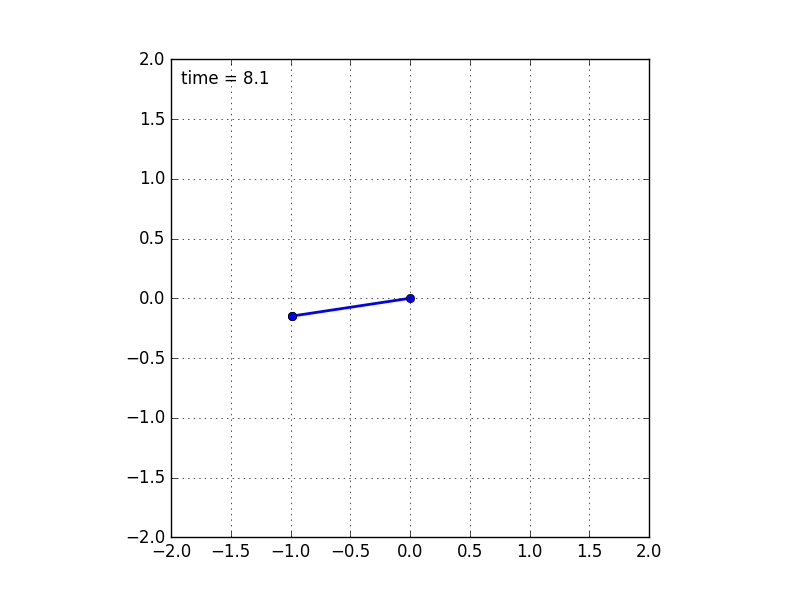
\includegraphics[width=7.5cm]{Pendulo90.png}
\caption{Imagen de Animación de péndulo con ángulo inicial 90.}
\end{figure}

\begin{figure}[H]
\centering
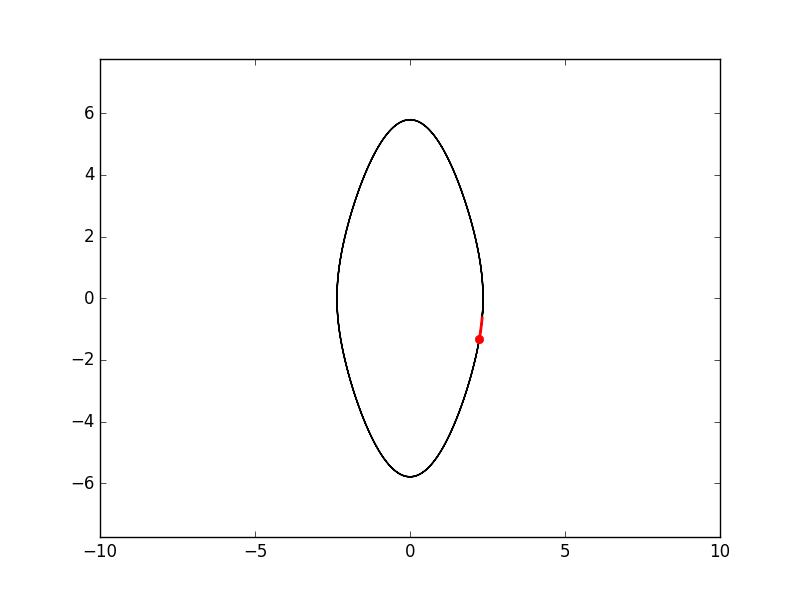
\includegraphics[width=7cm]{Fase135.png}
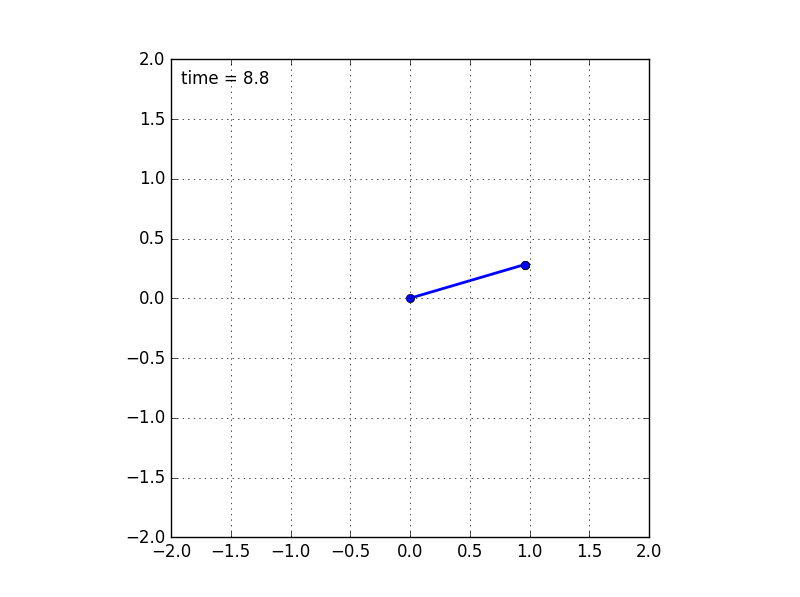
\includegraphics[width=7.5cm]{Pendulo135.png}
\caption{Imagen de Animación de péndulo con ángulo inicial 135.}
\end{figure}

\begin{figure}[H]
\centering
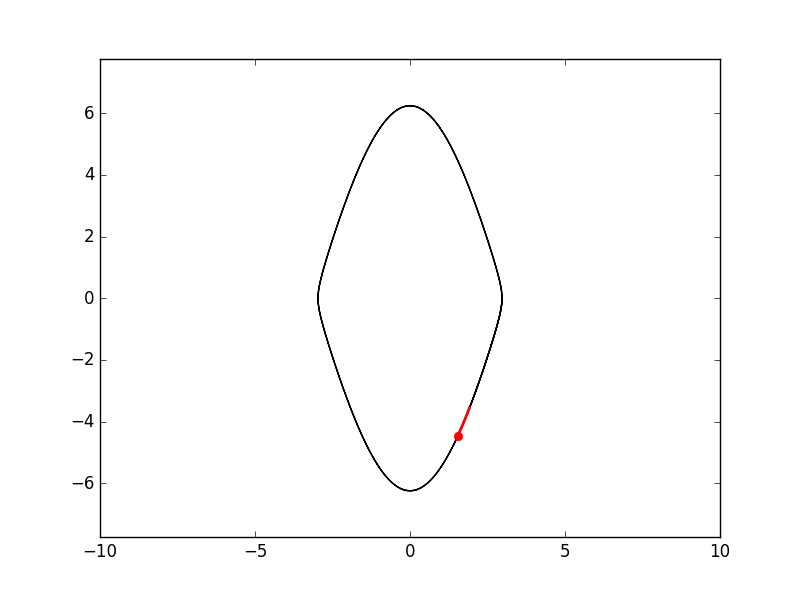
\includegraphics[width=7cm]{Fase170.png}
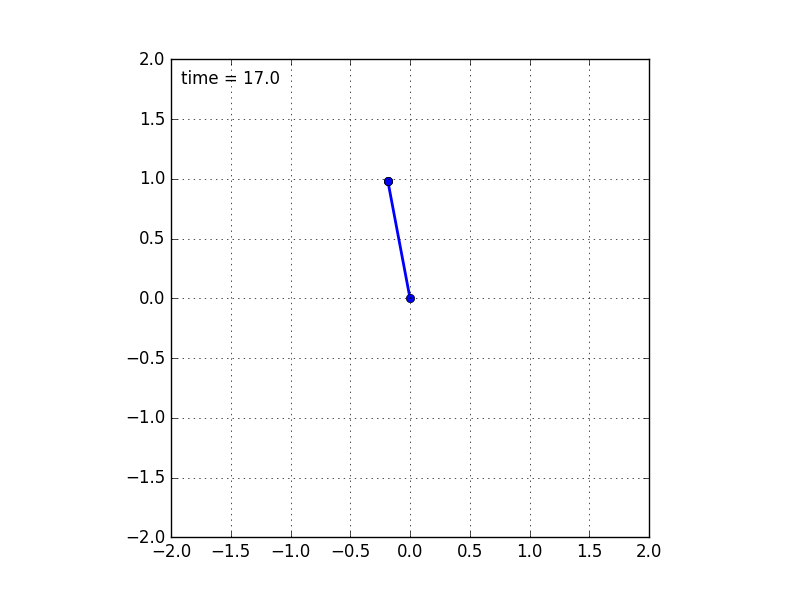
\includegraphics[width=7.5cm]{Pendulo170.png}
\caption{Imagen de Animación de péndulo con ángulo inicial 170.}
\end{figure}

\begin{figure}[H]
\centering
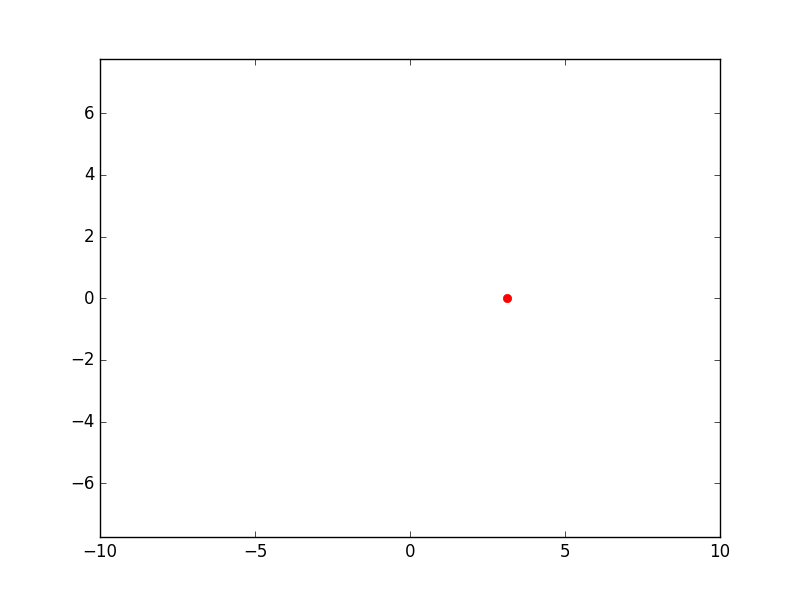
\includegraphics[width=7cm]{Fase180.png}
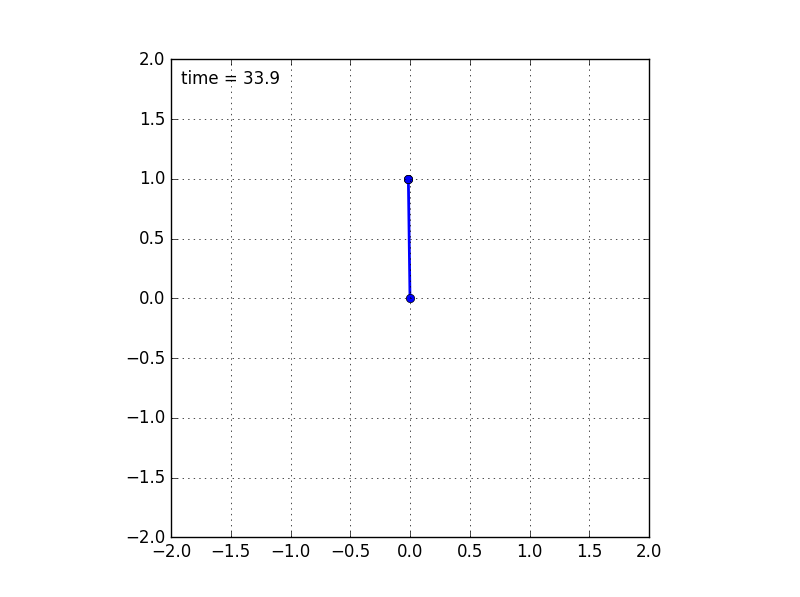
\includegraphics[width=7.5cm]{Pendulo180.png}
\caption{Imagen de Animación de péndulo con ángulo inicial 180.}
\end{figure}

\begin{figure}[H]
\centering
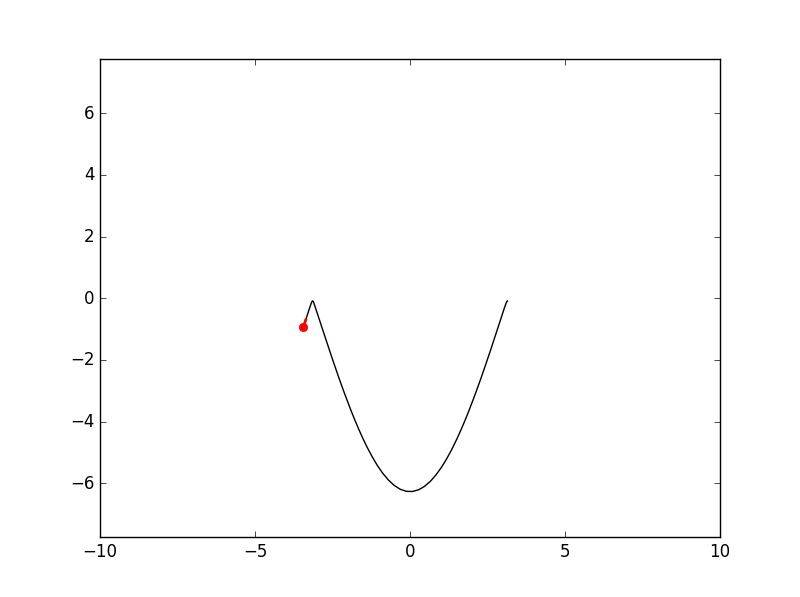
\includegraphics[width=7cm]{FaseFull2.png}
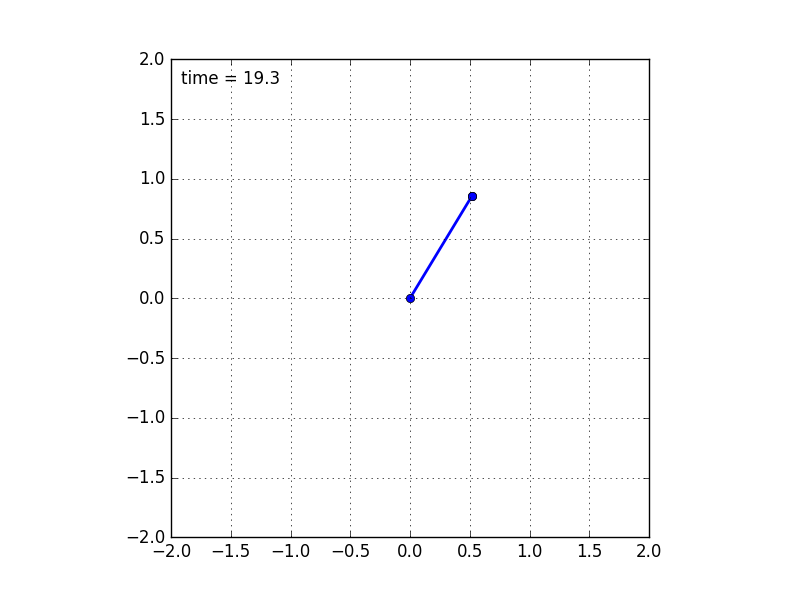
\includegraphics[width=7.5cm]{PenduloFull2.png}
\caption{Imagen de Animación de péndulo con apenas energía para completar la vuelta.}
\end{figure}

\begin{figure}[H]
\centering
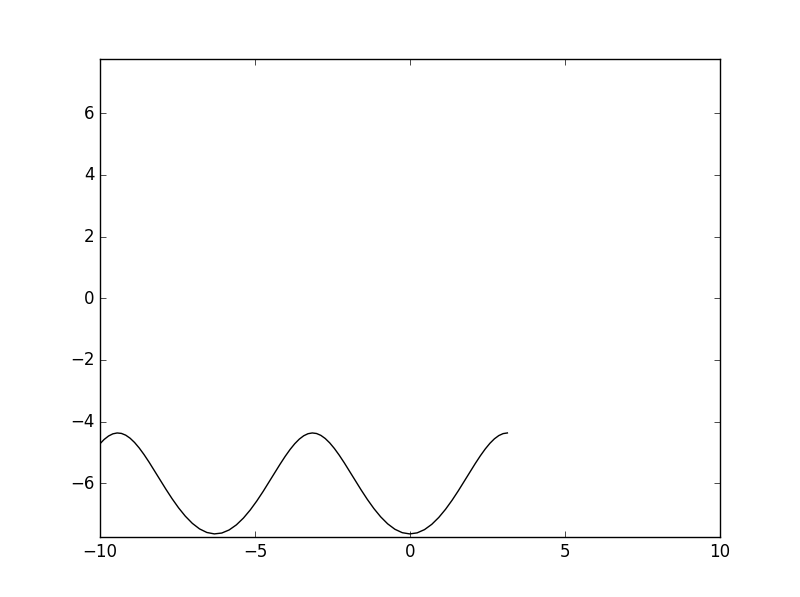
\includegraphics[width=7cm]{FaseFull1.png}
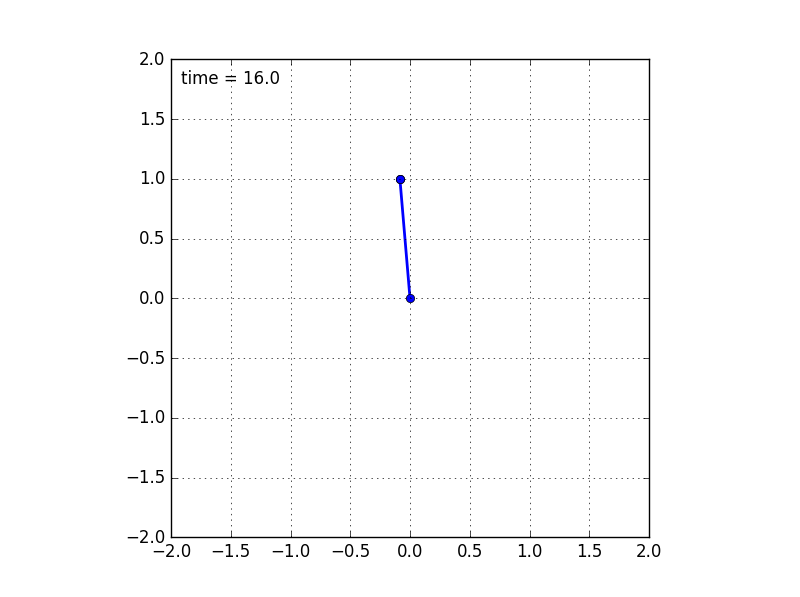
\includegraphics[width=7.5cm]{PenduloFull1.png}
\caption{Imagen de Animación de péndulo con suficiente energía para completar la vuelta.}
\end{figure}

Se adjuntaron vídeos de las animaciones de cada uno de los casos.
%============================================================================================================
\pagebreak

\begin{thebibliography}{6}
\bibitem{PendWiki}
	Wikipedia,(2016)
	\emph{Pendulum (mathematics)}. Recuperado de \url{https://en.wikipedia.org/wiki/Pendulum\_\%28mathematics\%29}

\bibitem{cod1}
	Vanderplas, J.(2012)
	\emph{Matplotlib Animation Tutorial} Recuperado de \url{https://jakevdp.github.io/blog/2012/08/18/matplotlib-animation-tutorial/}

\bibitem{cod2}
	Matplotlib(2012)
	\emph{animation example code: subplots.py} Recuperado de \url{http://matplotlib.org/examples/animation/subplots.html}

\bibitem{Act}
Lizárraga, C. (2016)
\emph{Actividad 10 (2016-1)}. Recuperado de \url{http://computacional1.pbworks.com/w/page/107247876/Actividad\%2010\%20(2016-1)}
\end{thebibliography}

\end{document}